% Home page cover: the front page of a datasheet for an imaginary part, EEP-101.
% The signal pins name the parts of the guide in order, so the figure is also a map.
% Page 1 is the full sheet (containers 34rem and wider). Page 2 is the mobile
% crop: header, package and pin table. Colors are fixed hex values here; the
% theme script swaps each one for a site token after export.
\documentclass[tikz,border=1pt,dvisvgm]{standalone}
\def\pgfsysdriver{pgfsys-dvisvgm.def}
\usepackage{fontspec}
\setmainfont{SourceSerif4SmText}[
  Path = ../../../.cache/fonts/source-serif-4.005_Desktop/OTF/,
  Extension = .otf,
  UprightFont = *-Regular,
  ItalicFont = *-It,
  BoldFont = *-Semibold,
  BoldItalicFont = *-SemiboldIt,
  Numbers = Lining]
\usepackage{xcolor,colortbl,array}
\definecolor{ink}{HTML}{16233A}    % --eep-dg-ink
\definecolor{inktwo}{HTML}{424D63} % --eep-ink-2
\definecolor{silver}{HTML}{838C9A} % --eep-dg-mute, lines only
\definecolor{tint}{HTML}{F1F2F3}   % --eep-dg-tint, fills only
\definecolor{surface}{HTML}{FFFFFF}% --eep-dg-fill
\usetikzlibrary{arrows.meta,calc,positioning}
\tikzset{every picture/.style={line width=0.5pt, draw=ink, text=ink}}
\arrayrulecolor{silver}
\setlength{\arrayrulewidth}{0.5pt}
\renewcommand{\arraystretch}{1.25}
% Type scale. Nothing is set under 8pt.
\newcommand{\txt}{\fontsize{8}{10}\selectfont}
\newcommand{\hd}[1]{{\fontsize{9.5}{11}\selectfont\bfseries #1}}
\newcommand{\colhd}[1]{{\bfseries\fontsize{8}{10}\selectfont #1}}
\newcommand{\subs}[1]{\textsubscript{#1}}
\newcommand{\var}[1]{\textit{#1}}
\newcommand{\bul}{\makebox[0.9em][l]{\textbullet}}
% A bullet item with a hanging indent, so a wrapped line lines up under the text.
\newcommand{\bi}[1]{\par\noindent\hangindent=0.9em\hangafter=1\bul #1\par}
\newcommand{\docno}{EEPS101 \,–\, NOVEMBER 2026}

% ---------- Package drawing: DIP-8, top view, true proportions ----------
% 1 mm = \mm. 2.54 mm pitch, 7.62 mm row spacing, 6.35 x 9.81 mm body.
\newcommand{\mm}{0.30cm}
\newsavebox{\pkgbox}
\sbox{\pkgbox}{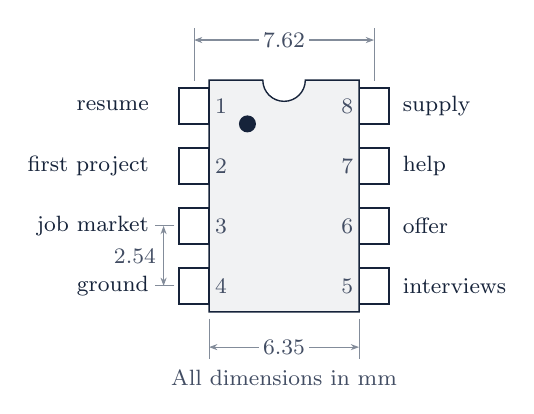
\begin{tikzpicture}[x=\mm, y=\mm, line width=0.5pt]
  \def\bw{3.175} \def\bl{4.905}
  % Leads: 1.52 mm wide, centered on the 7.62 mm rows.
  \foreach \i/\y in {1/3.81, 2/1.27, 3/-1.27, 4/-3.81} {
    \draw[fill=surface] (-4.445,\y-0.76) rectangle (-\bw,\y+0.76);
    \draw[fill=surface] (\bw,\y-0.76) rectangle (4.445,\y+0.76);
  }
  % Body, pin-1 notch and dot.
  \draw[fill=tint] (-\bw,-\bl) -- (-\bw,\bl) -- (-0.9,\bl) arc[start angle=180, end angle=360, radius=0.9] -- (\bw,\bl) -- (\bw,-\bl) -- cycle;
  \fill[ink] (-1.55,3.05) circle[radius=0.36];
  % Pin numbers inside, names outside.
  \foreach \i/\y/\name in {1/3.81/resume, 2/1.27/first project, 3/-1.27/job market, 4/-3.81/ground} {
    \node[anchor=west, inner sep=0pt, text=inktwo] at (-2.95,\y) {\txt\i};
    \node[anchor=east, inner sep=0pt] at (-5.7,\y) {\txt\name};
  }
  \foreach \i/\y/\name in {8/3.81/supply, 7/1.27/help, 6/-1.27/offer, 5/-3.81/interviews} {
    \node[anchor=east, inner sep=0pt, text=inktwo] at (2.95,\y) {\txt\i};
    \node[anchor=west, inner sep=0pt] at (5.0,\y) {\txt\name};
  }
  \tikzset{dim/.style={draw=silver, line width=0.4pt, {Stealth[length=3pt,width=2.2pt]}-{Stealth[length=3pt,width=2.2pt]}},
           ext/.style={draw=silver, line width=0.4pt}}
  % 7.62 row spacing, above.
  \draw[ext] (-3.81,4.57+0.3) -- (-3.81,7.1);
  \draw[ext] (3.81,4.57+0.3) -- (3.81,7.1);
  \draw[dim] (-3.81,6.6) -- (3.81,6.6) node[midway, fill=surface, inner sep=1.5pt, text=inktwo] {\txt 7.62};
  % 6.35 body width, below.
  \draw[ext] (-\bw,-\bl-0.3) -- (-\bw,-6.9);
  \draw[ext] (\bw,-\bl-0.3) -- (\bw,-6.9);
  \draw[dim] (-\bw,-6.4) -- (\bw,-6.4) node[midway, fill=surface, inner sep=1.5pt, text=inktwo] {\txt 6.35};
  % 2.54 pitch, between the leads of pins 3 and 4.
  \draw[ext] (-4.445-0.2,-1.27) -- (-5.45,-1.27);
  \draw[ext] (-4.445-0.2,-3.81) -- (-5.45,-3.81);
  \draw[dim] (-5.1,-1.27) -- (-5.1,-3.81);
  \node[anchor=east, inner sep=0pt, text=inktwo] at (-5.4,-2.54) {\txt 2.54};
  \node[anchor=north, inner sep=0pt, text=inktwo] at (0,-7.35) {\txt All dimensions in mm};
\end{tikzpicture}}

% ---------- Pieces shared by both pages ----------
% #1: sheet width.
\newcommand{\topbar}[1]{%
  \draw[line width=0.6pt] (0,0) -- (#1,0);
  \node[anchor=north west, inner sep=0pt] at (0,-0.16) {\hd{eeprep}};
  \node[anchor=north east, inner sep=0pt, align=right] at (#1,-0.16) {\txt\bfseries EEP-101\\[1pt] \txt\color{inktwo}\docno};
  \draw[line width=0.6pt] (0,-0.95) -- (#1,-0.95);
}
\newcommand{\titleblock}[2]{% #1 width, #2 y
  \node[anchor=north west, inner sep=0pt, text width=#1 cm, align=flush left] (title) at (0,#2)
    {{\fontsize{13}{15.5}\selectfont\bfseries EEP-101 General-Purpose Intern}\\[3pt]\txt\color{inktwo}Preliminary};
}
\newcommand{\footer}[2]{% #1 width, #2 a coordinate in parentheses
  \coordinate (fy) at #2;
  \draw[draw=silver] (0,0 |- fy) -- (#1,0 |- fy);
  \node[anchor=north west, inner sep=0pt, text=inktwo] at ($(0,0 |- fy)+(0,-0.12)$) {\txt\docno};
  \node[anchor=north east, inner sep=0pt, text=inktwo] at ($(#1,0 |- fy)+(0,-0.12)$) {\txt 1};
}
% Pin functions table. #1: description column width.
\newcommand{\pintable}[1]{%
  \txt
  \begin{tabular}{@{\hspace{3pt}}>{\raggedright}p{3.9em}>{\raggedright}p{6.0em}>{\raggedright}p{2.8em}>{\raggedright\arraybackslash}p{#1}@{\hspace{3pt}}}
  \hline
  \rowcolor{tint}\colhd{PIN NO.} & \colhd{NAME} & \colhd{TYPE} & \colhd{DESCRIPTION} \\ \hline
  1 & resume & I & Resume, one page \\ \hline
  2 & first project & I & Hardware project \\ \hline
  3 & job market & I & Openings and timing \\ \hline
  4 & ground & G & Coursework basics \\ \hline
  5 & interviews & I/O & Technical interviews \\ \hline
  6 & offer & O & Internship offer \\ \hline
  7 & help & I & Job boards and contacts \\ \hline
  8 & supply & P & Rest and routine \\ \hline
  \end{tabular}%
}

\begin{document}
% =================== Page 1: full sheet ===================
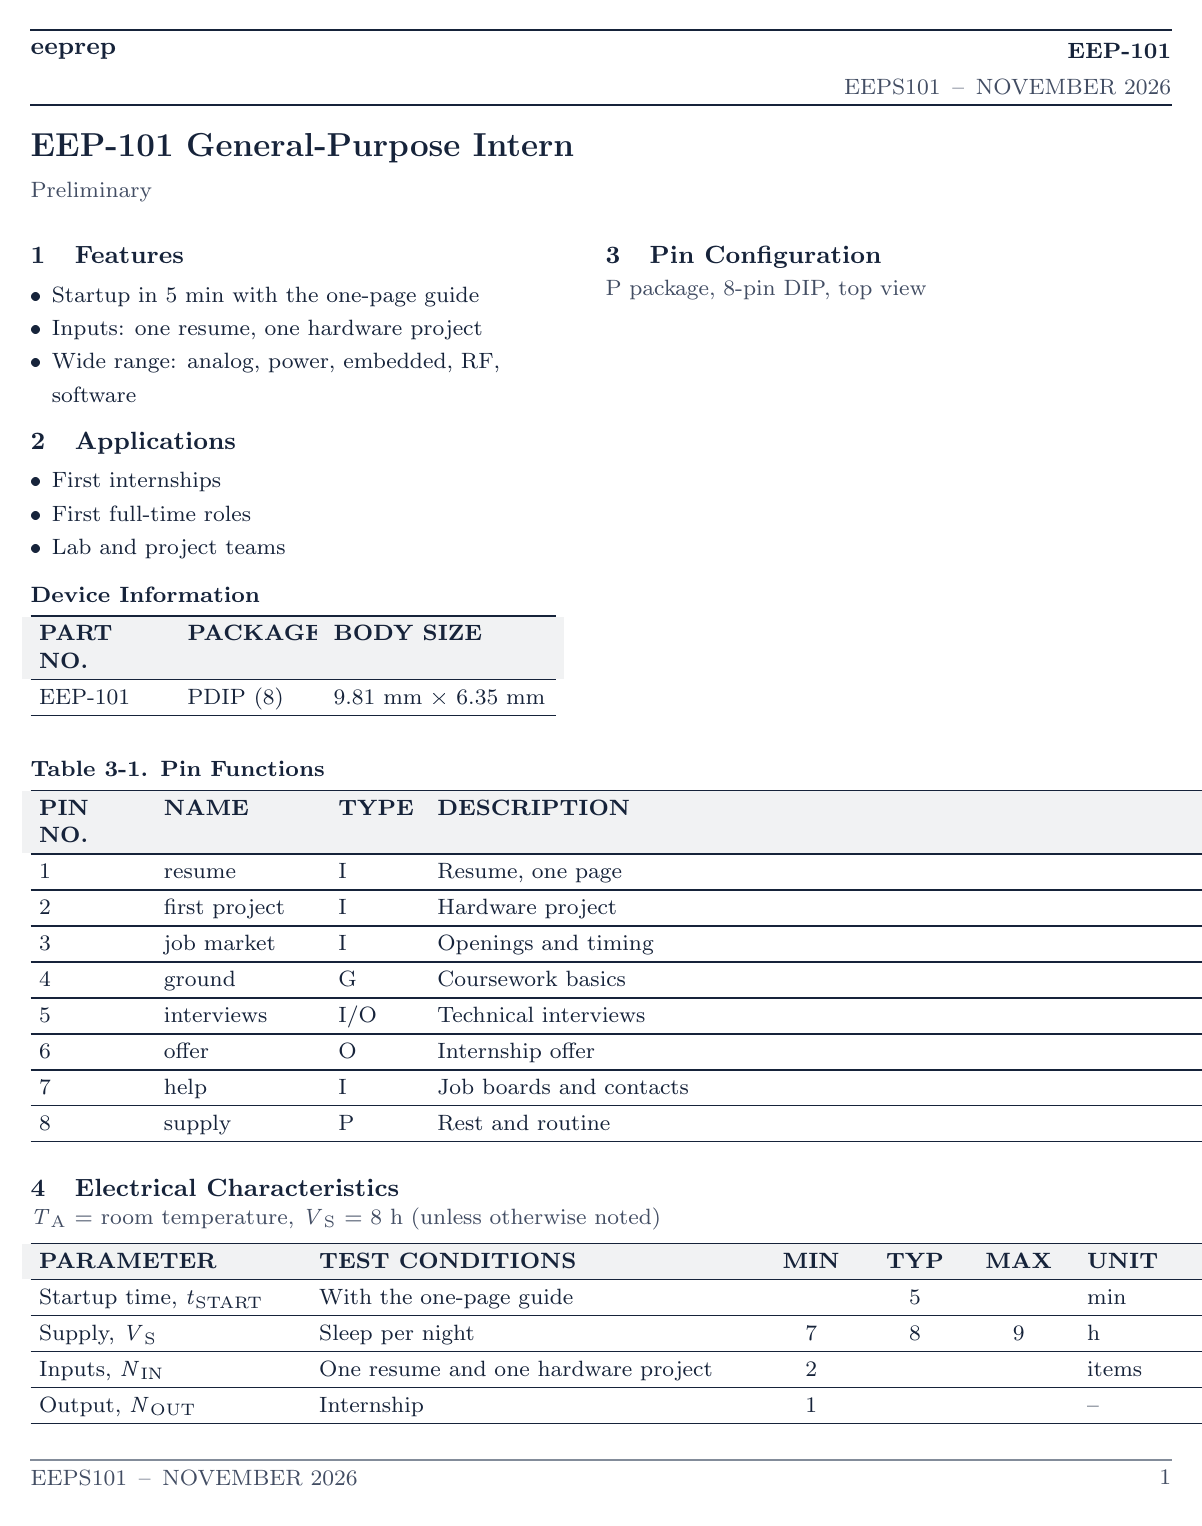
\begin{tikzpicture}
\def\W{14.5}
\color{ink}
\topbar{\W}
\titleblock{\W}{-1.3}
% Left column: features, applications, device information.
\node[anchor=north west, inner sep=0pt, text width=6.4cm, align=flush left, font=\fontsize{8}{12}\selectfont] (feat) at ($(title.south west)+(0,-0.55)$) {%
  \parskip=0pt
  \noindent\hd{1\quad Features}\par\vspace{2pt}
  \bi{Startup in 5 min with the one-page guide}
  \bi{Inputs: one resume, one hardware project}
  \bi{Wide range: analog, power, embedded, RF, software}
  \vspace{5pt}
  \noindent\hd{2\quad Applications}\par\vspace{2pt}
  \bi{First internships}
  \bi{First full-time roles}
  \bi{Lab and project teams}};
\node[anchor=north west, inner sep=0pt] (dih) at ($(feat.south west)+(0,-0.34)$) {\txt\bfseries Device Information};
\node[anchor=north west, inner sep=0pt] (di) at ($(dih.south west)+(0,-0.15)$) {\txt
  \begin{tabular}{@{\hspace{3pt}}>{\raggedright}p{4.9em}>{\raggedright}p{4.8em}>{\raggedright\arraybackslash}p{9.1em}@{\hspace{3pt}}}
  \hline
  \rowcolor{tint}\colhd{PART NO.} & \colhd{PACKAGE} & \colhd{BODY SIZE} \\ \hline
  EEP-101 & PDIP (8) & 9.81 mm × 6.35 mm \\ \hline
  \end{tabular}};
% Right column: pin configuration.
\node[anchor=north west, inner sep=0pt] (pchead) at ($(title.south west)+(7.3,-0.55)$) {\hd{3\quad Pin Configuration}};
\node[anchor=north west, inner sep=0pt, text=inktwo] (pcsub) at ($(pchead.south west)+(0,-0.12)$) {\txt P package, 8-pin DIP, top view};
\node[anchor=north, inner sep=0pt] (pkgnode) at ($(7.3,0 |- pcsub.south)+(3.6,-0.35)$) {\usebox{\pkgbox}};
% Full width: pin functions, then electrical characteristics.
\path let \p1=(di.south), \p2=(pkgnode.south) in coordinate (t1) at (0,{min(\y1,\y2)-0.55cm});
\node[anchor=north west, inner sep=0pt] (pfh) at (t1) {\txt\bfseries Table 3-1. Pin Functions};
\node[anchor=north west, inner sep=0pt] (pf) at ($(pfh.south west)+(0,-0.15)$) {\pintable{32.8em}};
\node[anchor=north west, inner sep=0pt] (ech) at ($(pf.south west)+(0,-0.45)$) {\hd{4\quad Electrical Characteristics}};
\node[anchor=north west, inner sep=0pt, text=inktwo] (ecs) at ($(ech.south west)+(0,-0.12)$) {\txt\var{T}\subs{A} = room temperature, \var{V}\subs{S} = 8 h (unless otherwise noted)};
\node[anchor=north west, inner sep=0pt] (ec) at ($(ecs.south west)+(0,-0.15)$) {\txt
  \begin{tabular}{@{\hspace{3pt}}>{\raggedright}p{10.5em}>{\raggedright}p{18.0em}>{\centering}p{3em}>{\centering}p{3em}>{\centering}p{3em}>{\raggedright\arraybackslash}p{5.1em}@{\hspace{3pt}}}
  \hline
  \rowcolor{tint}\colhd{PARAMETER} & \colhd{TEST CONDITIONS} & \colhd{MIN} & \colhd{TYP} & \colhd{MAX} & \colhd{UNIT} \\ \hline
  Startup time, \var{t}\subs{START} & With the one-page guide & & 5 & & min \\ \hline
  Supply, \var{V}\subs{S} & Sleep per night & 7 & 8 & 9 & h \\ \hline
  Inputs, \var{N}\subs{IN} & One resume and one hardware project & 2 & & & items \\ \hline
  Output, \var{N}\subs{OUT} & Internship & 1 & & & – \\ \hline
  \end{tabular}};
\footer{\W}{($(ec.south)+(0,-0.45)$)}
\pgfresetboundingbox\path (-0.03,0.03) rectangle ($(\W,0 |- fy)+(0.03,-0.48)$);
\end{tikzpicture}

% =================== Page 2: mobile crop ===================
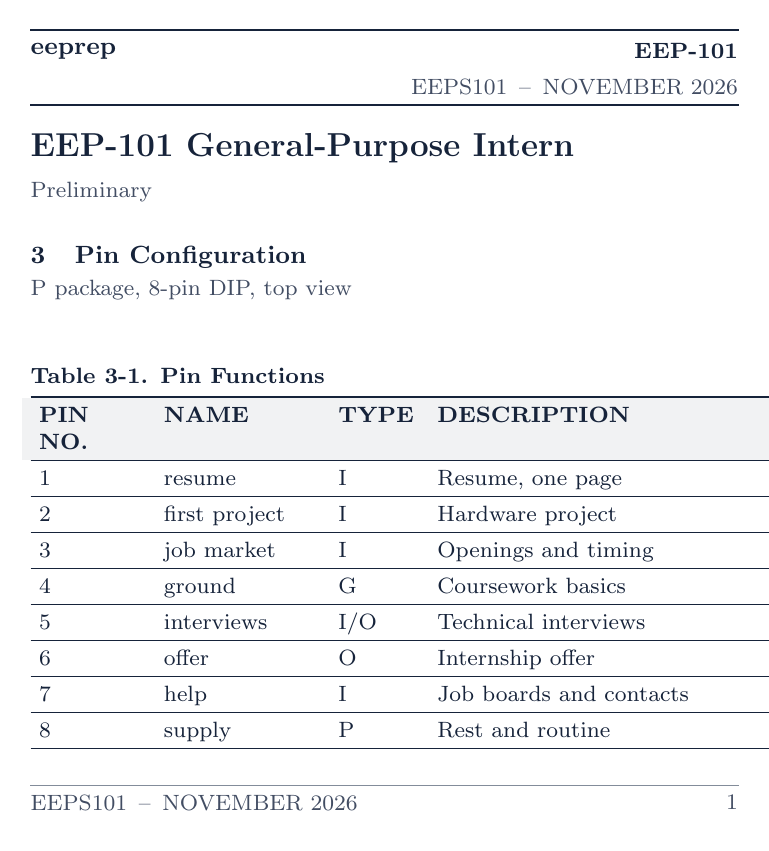
\begin{tikzpicture}
\def\W{9.0}
\color{ink}
\topbar{\W}
\titleblock{\W}{-1.3}
\node[anchor=north west, inner sep=0pt] (pchead) at ($(title.south west)+(0,-0.55)$) {\hd{3\quad Pin Configuration}};
\node[anchor=north west, inner sep=0pt, text=inktwo] (pcsub) at ($(pchead.south west)+(0,-0.12)$) {\txt P package, 8-pin DIP, top view};
\node[anchor=north, inner sep=0pt] (pkgnode) at ($(\W/2,0 |- pcsub.south)+(0,-0.35)$) {\usebox{\pkgbox}};
\node[anchor=north west, inner sep=0pt] (pfh) at ($(0,0 |- pkgnode.south)+(0,-0.45)$) {\txt\bfseries Table 3-1. Pin Functions};
\node[anchor=north west, inner sep=0pt] (pf) at ($(pfh.south west)+(0,-0.15)$) {\pintable{14.1em}};
\footer{\W}{($(pf.south)+(0,-0.45)$)}
\pgfresetboundingbox\path (-0.03,0.03) rectangle ($(\W,0 |- fy)+(0.03,-0.48)$);
\end{tikzpicture}
\end{document}
